\documentclass[runningheads,a4paper]{llncs}
\usepackage{amssymb}
\setcounter{tocdepth}{3}
\usepackage{graphicx}
\usepackage{algorithmic}
\usepackage{algorithm}

\usepackage{url}
\urldef{\mailsa}\path|{adrianr, davidc, jayen, bernhardh}@cse.unsw.edu.au|  
\newcommand{\keywords}[1]{\par\addvspace\baselineskip
\noindent\keywordname\enspace\ignorespaces#1}

\begin{document}

\mainmatter

\title{Fast Object Detection with Foveated Imaging and Virtual Saccades on Resource Limited Robots}

\titlerunning{Fast Object Detection}

\author{Adrian Ratter \and David Claridge\and \\
    Jayen  Ashar \and Bernhard Hengst}

%\authorrunning{Adrian Ratter et al.}

\institute{School of Computer Science and Engineering,\\
University of New South Wales, UNSW Sydney 2052 Australia}

\toctitle{Fast Object Detection Using Foveated and Virtual Saccades on a Resource Limited Robot}
%\tocauthor{Adrian Ratter}
\maketitle


\begin{abstract}
This paper describes the use of foveated imaging and virtual saccades to
identify visual objects using both colour and edge features. Vision processing
is a resource hungry operation at the best of times. When the demands require
robust, real-time performance with a limited embedded processor, the challenge
is significant. Our domain of application is the RoboCup Standard Platform
League soccer competition using the Aldebaran Nao robot. We describe algorithms
that use a combination of down-sampled colour images and high-resolution
edge-detection to identify objects in varying lighting conditions. Optimised to
run in real time on autonomous robots, these techniques can potentially be
applied in other resource limited domains. 
\end{abstract}


\section{Introduction}

Real-time identification of objects in a video feed is a significant research
area in robotics, and forms the major component of many perception systems. For
the rich environments we encounter in everyday life this is still an open
research problem.  RoboCup Soccer\cite{robocupurl} is an international research
and education initiative that constrains the environment to a soccer field with
a limited number of objects, namely a ball, field, goal-posts, and other
robots. Vision algorithms are able to exploit these constraints, but face
significant challenges.

Small, mobile robots are limited in their processing power. Vision
needs to share this limited resource with other functions such as
world-modelling and behaviour generation. Success in soccer also depends on the
speed at which robots can react. A major challenge is for the vision system to
deliver real-time object recognition at the full frame-rate and still leave
resources for the other functions. 

Colour cameras provide a high native pixel resolution in a three
dimensional colour space. It is taxing on resources to process the image in its
full resolution. When objects are relatively far away, and appear small in the
visual field, we would like to take advantage of the higher resolution. 

\begin{figure}
\centering
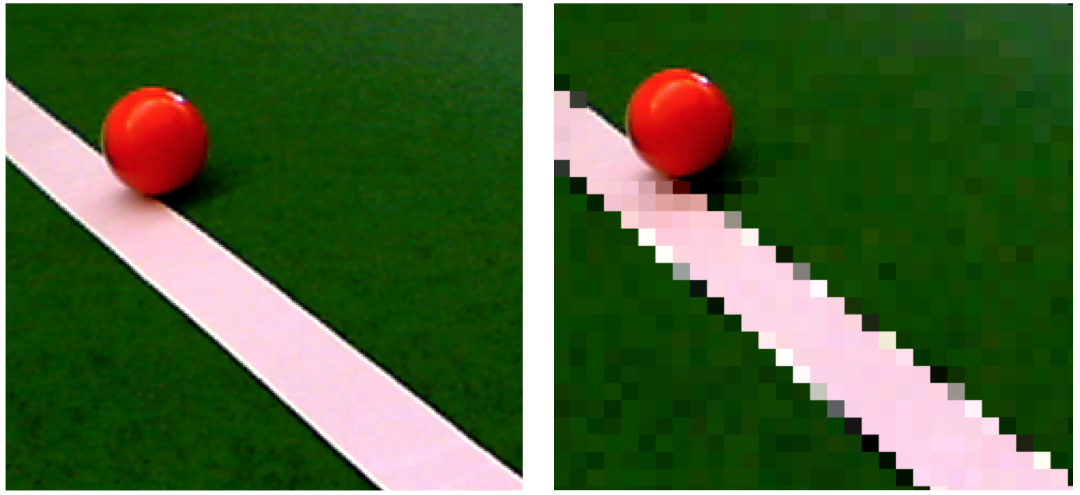
\includegraphics[width=0.5\textwidth]{figures/figFov}
\caption{Foveated imaging. Original Image (left). Virtual fovea centred on a ball (right) } \label{figFov}
\end{figure}

The human eye has a region with maximum acuity in the centre of the macular know
as the fovea. Motivated by this physiology the above dilemma can be addressed by
varying the resolution and processing across the image according to one or more
points of fixation. This technique is called \emph{foveated imaging}. The fovea
provides a high resolution image, but a very narrow field-of-view.
\emph{Peripheral vision} is provided by the image outside the foveal regions at
lower resolution. These ideas have been used in computer vision inspiring both
software and hardware solutions.\cite{724279} Figure~\ref{figFov} shows an
image at full camera resolution on the left and a foveated image on the right,
with the fovea saccaded and fixed on the ball. 

The RoboCup soccer environments are characterised by objects with distinct colours. It is not surprising that algorithms to date have largely used colour to identify objects. Organisers have gradually increased the vision challenge by progressively removing crutches such as walls, beacons and coloured goal-posts. In particular, the practice of providing special high luminescent and uniform lighting has been discontinued and robots need to cope with whatever lighting is provided by the venue. Lighting often changes during games as audience numbers fluctuate creating varying overshadowing conditions during the game. One solution is for vision to rely less on colour and more on shape cues. 

The contribution of this paper is a vision system that addresses the above needs with the following characterstics:
\begin{enumerate}
\item A peripheral vision system to locate salient features. A novelty is the detection of field-edges for localisation using the saliency image alone.   
\item Employing foveated imaging techniques to limit resource usage.
\item Relying more on edges and reducing the dependence on colour.
\item Meeting real-time requirements running close to the full frame-rate.
\end{enumerate}

The application of these methods have broad applicability. We describe them in
the context of the Standard Platform League that uses the small humanoid Nao
robot from Aldebaran Robotics. The rules of the league disallow external
processing or any modification to the machine. The robots' embedded computer is
limited to an AMD Geode LX 800 processor running at a modest 500MHz. The playing
area of the soccer field is currently 4 by 6 meters with colour coded open
goals. A team-size of three robots was used in 2010 and this will increase to
four in 2011. The ball is a standard orange coloured street hockey ball. Each
robot has two CCD $640 \times 480$ pixel cameras in its head (although only one
can be used at a time).  

In the rest of this paper we will describe the down-sampled ``saliency" frames
that are used to identify possible locations of various objects on the field.
The saliency image is used to find field-edges to aid in the localisation of
the robot. We next show how the saliency image leads to virtual saccades to
multiple points of fixation representing interest regions corresponding to the
ball and goals. Multi-modal colour and edge data at high resolution is used at
these foveal points in the image, achieving both high accuracy and high
efficiency. 

This approach was implemented by the UNSW team \emph{rUNSWift} for the Standard Platform League in  RoboCup World Competition in Singapore in 2010, for both the technical challenges and the soccer tournament. The University of New South Wales (UNSW) placed first in the technical challenges and second in the soccer competition against 23 other international teams.

\section{Saliency Scan}

In order to achieve our goal of identifying areas of interest in the image as
fast as possible, the first step of the vision pipeline is to subsample the
image in a regular grid pattern. We reduce the image size by a factor of $n$ for
each of the two image dimensions. We have chosen $n=4$ for the 2010 competition
to make optimally use of machine cycles, but experiments show that $n=8$ is
still acceptable if we wish to use fewer resources. The advantage is that the
number of pixels to be processed is reduced by a factor of $n^2$. By mapping
every 4th pixel in the raw $640 \times 480$ image we derive a $160 \times 120$
pixel resolution ``saliency image" giving a 16 fold reduction in image size. For
$n=8$ the saliency vision processing load is reduced by 98.4\%.
Figure~\ref{figFov} (right) shows a down-sampled part-image of the green field,
field-line, and ball for $n=8$. A rectangle containing the ball shows a virtual
fovea region at the original raw resolution. 

\begin{figure}
\centering
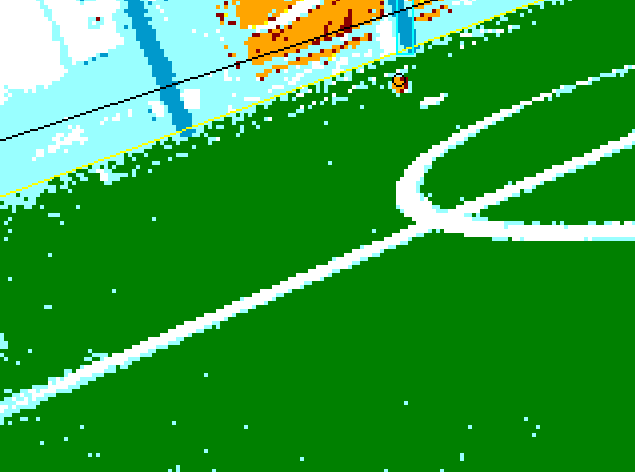
\includegraphics[width=0.37\textwidth]{figures/figSal}
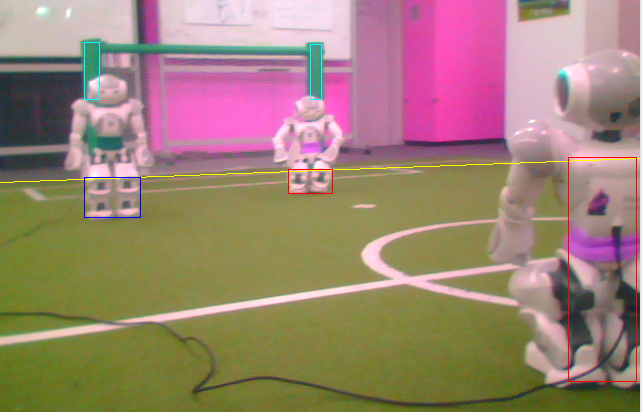
\includegraphics[width=0.45\textwidth]{figures/robotDetectionScreenshot.png}
\caption{Colour classified saliency image at $160 \times 120$ resolution  ie.
$n=4$ (left). Goal and robot regions identified
during the region detection process (right).} \label{figSal}
\end{figure}

Each pixel that is part of the saliency image is colour classified before it is stored. The colours
are calibrated off-line using a weighted kernel classification algorithm
developed for previous Robocup competitions.\cite{kimcuongpham} This is a
nearest neighbour algorithm where each training sample increases a weighting for
a particular YUV value toward the classified colour. The classifier is able to
generalise to unseen data as neighbouring values in colour-space, within a fixed
Euclidean radius, have their weights increased at an exponentially decreasing
rate. The kernel file is used to generate a constant-time lookup table on the
robot at runtime. The colours calibrated are orange (the ball), green (the
field), white (the field-lines and parts of the robots), yellow (the yellow
goals), red (the pink band worn by robots on the red team), blue (the blue
goals and the blue band worn by robots on the blue team) and background (to remove background objects with a similar colour to the ones used on a Robocup field).
%Do we calibrate background or black?

%As the saliency image is generated for every visual frame at 30 fps, any further
%optimisation is desirable. We analysed the compiler-generated assembly code to
%find optimisation opportunities. The main optimisations are as follows: 

%jayen reducing detail as the details are implementation specific
%\begin{itemize}
%  \item Reducing the amount of memory used
%  \item Reducing the number of memory accesses
%  \item Reducing the number of local variables used (thereby reducing the
%number of variables in memory)
%  \item Reducing the number of calculations required for image access by using
%pointer arithmetic instead of array indexing
%\end{itemize}

In the following sections we will describe how the colour calibrated saliency scan can be used to rapidly identify objects of interest in the image. 
%In addition, while the saliency scan is being generated, histograms in the $x$ and $y$-axes for the yellow and blue colours are generated. The maxima of these histograms can be found efficiently, allowing the rest of the vision system to quickly identify the likely locations of the goal posts, so only these locations are analysed at the native resolution.
%Need to define ``major'' field-space colors.  only blue and yellow histograms
%are generated, while I consider green and white to be major field-space colors.


\section{Field-Edge Detection Using the Saliency Scan}

To further reduce the amount of the image that has to be processed for object
identification, and to assist with localisation, the edges of the green field
are detected using the Saliency Scan image. After vertically scanning the saliency image to detect points on the
%In 2009 B-Human used a convex hull
%algorithm to exclude areas above the field-edge\cite{thomas09code}, which
%achieves the first goal of reducing the area of the image to be processed. In
%2010 rUNSWift used a similar method of vertical scanning to detect points on the
edge of the field, multiple
iterations of the RANSAC algorithm\cite{Fischler:1981:RSC:358669.358692} are
used to find straight lines. When two field-edge lines are detected, the
possible positions of the robot are reduced to 4 hypotheses.

\begin{figure}
\centering
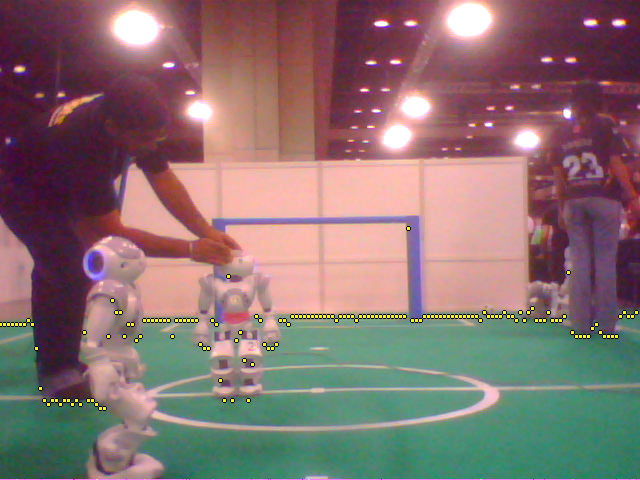
\includegraphics[width=0.4\textwidth]{figures/EdgeDetection_OneLinePoints}
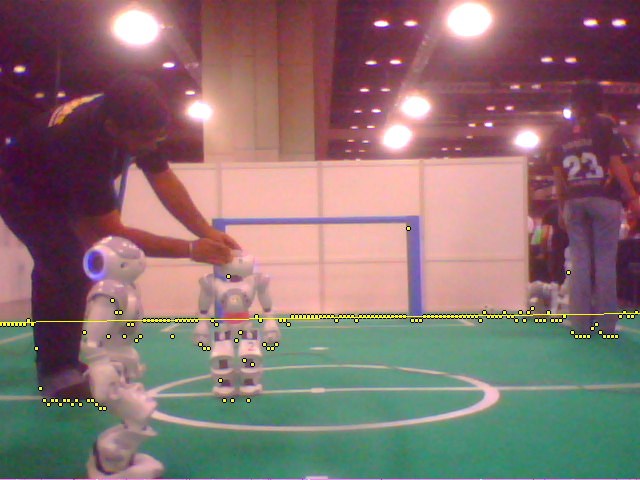
\includegraphics[width=0.4\textwidth]{figures/EdgeDetection_OneLinePointsAndLine}
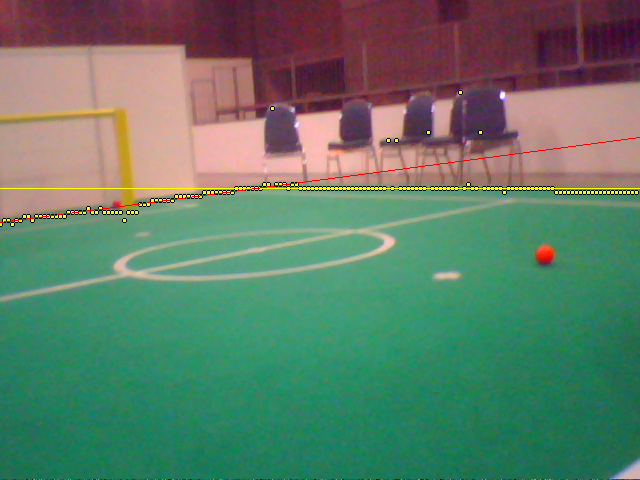
\includegraphics[width=0.4\textwidth]{figures/EdgeDetection_TwoLines}
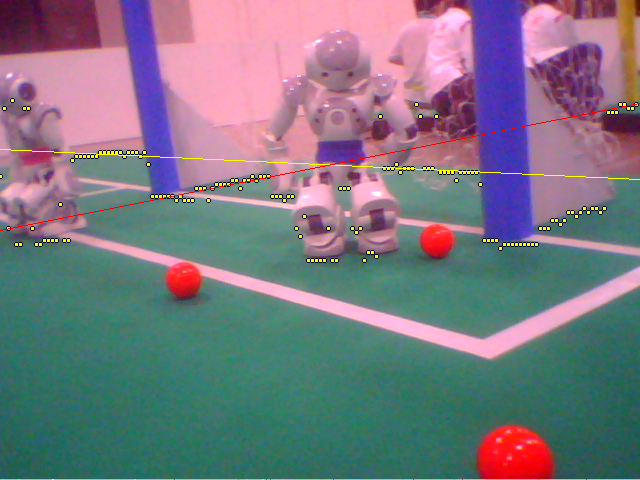
\includegraphics[width=0.4\textwidth]{figures/EdgeDetection_PostTriangleError}
\caption{Candidate points for a field-edge line (top-left). Line found by
performing RANSAC on candidate points (top-right). Lines found by performing
RANSAC twice on the candidate points (bottom-left). False-positive field-edge
(bottom-right) .} \label{figEdge}
\end{figure}

Initially, the first green pixel in each column of the saliency scan is
recorded, by scanning vertically from the horizon down (the horizon is found by
using kinematics; by using the robot dimensions and joint angles to calculate what pixels in the image correspond to the horizon \cite{cse10rUNSWift2010}) -
Figure~\ref{figEdge} (top-left). %top-left of figure has no horizon
Secondly, the pixels are fit to a line of
the form $t_1x + t_2y + t_3 = 0$ with the RANSAC algorithm, to maximise the
number of points that fit a line - Figure~\ref{figEdge} (top-right). Finally,
the consensus set of the first line is removed from the candidate points, and
RANSAC is repeated, possibly finding a second line - Figure~\ref{figEdge}
(bottom-left). Figure~\ref{figEdge} (bottom-right) shows a false-positive for
one of the field-edges caused by the triangular goal-post support. Its effect is
rapidly filtered out with goal-post localisation information.

In addition to reducing the amount of the image to be scanned for objects to the
parts of the image below the field-edge, these field-edge observations were able
to be used to provide useful updates to the robot's estimated position on the
field.\cite{hengst10robocup}

\section{Finding Interest Points Using the Saliency Scan}

We scan the colour classified pixels underneath the field-edge to identify potential areas, or regions, that could represent important features, such as the ball, other robots, or field-lines. The contents of each of these regions are analysed to determine what objects they may represent. By only examining small areas of interest at the full resolution, this method of virtual saccades enabled us to greatly increase the run-time speed of the vision processing system.

Points of interest are found by scanning each column of the saliency scan image below the field-edge to identify runs of non-field green coloured pixels. For runs starting with orange (ball coloured) pixels, the run will finish when either a green, white, robot red or robot blue pixel is found, when a few unclassified pixels are found, or when the bottom of the image is reached. Alternatively, for runs starting with other colours, they will finish when either an orange pixel is found, when more than one green pixel in a row is found, or when the bottom of the image is reached. 

Run information is used to build regions. A run is connected to an existing region only if the following conditions are met: 
\begin{itemize}
\item{the last run added to the region is adjacent to the current run.}
\item{the region contains orange pixels (the colour of the ball) and the run also contains orange
pixels.}
\item{the run contains robot coloured pixels and the region does not and the
region is less than a certain width. This is to make sure any arms and legs that are protuding out from the robot's body are considered part of the region representing the robot.}
\item{the run contains no robot coloured pixels and the region does and the
difference between the x coordinate of the current run and the x coordinate of
the right most robot coloured pixel in the region is less than a certain
threshold. Similarly to the previous condition, this is desigend to amke sure a robot's arms and legs are added to the region representing the robot.}
\item{the length of the run is between 50\% and 200 \% of the average run length
of the region so far. This helps to separate runs representing field lines from runs representing robots.}
\end{itemize}

If no region is able to meet all these conditions, a new region is created for
the run. An array of pointers to regions containing runs from the previous
column is stored to avoid large numbers of regions slowing down processing. 
%The process is summarised in Algorithm~\ref{algReg}. 


%\begin{algorithm} [ht]
%    \caption{Region Building Algorithm} \label{algReg}
%    \begin{algorithmic}
%    \FORALL{$column\ \mathbf{in}\ saliencyScan$}
%    \FORALL{$row\ \mathbf{in}\ column$}
%    \IF{$row$ at end of a $run$}
%    \FORALL{$reg\ \mathbf{in}\ lastColumnRegions$}
%    \IF{$reg.startY > run.endY$} 
%    \STATE{\bf{continue}}
%    \ENDIF
%    \IF{$reg.endY \ge run.startY$}
%    \IF{conditions for joining $run$ to $reg$ are met}
%    \IF{$run$ hasn't been joined to a region yet}
%    \STATE{Join $run$ to $reg$}
%    \STATE{Add $reg$ to end of $thisColumnRegions$}
%    \ELSE
%    \STATE{Merge $reg$ with previous region $run$ joined}
%    \ENDIF
%    \ENDIF
%    \ELSE
%    \STATE{Remove $reg$ from $lastColumnRegions$} 
%    \ENDIF
%    \ENDFOR
%    \IF{$run$ has not been joined to a region}
%    \STATE{Create new region for $run$}
%    \STATE{Add new region to $thisColumnRegions$}
%    \ENDIF
%    \ENDIF
%    \ENDFOR
%    \STATE{Set $lastColumnRegions\ =\ thisColumnRegions$}
%    \STATE{Set $thisColumnRegions.size\ =\ 0$}
%    \ENDFOR
%\end{algorithmic}
%\end{algorithm}

Throughout this process, information about each run is collected for the region it joins. Information is collected such as the number of pixels of each colour in the region, the coordinates of the bounding box of the region, the average length of the runs in the regions, the start and end coordinates of each run in the region, and the bounding box of the robot colours in the region to be stored. This information is then used to identify what object (if any) the region is most likely to contain.

The initial object classification is performed by examining the colours, shape
and location of each region to determine if the region is more likely to contain
a ball, field-line, robot, or just be noise, such as noise from an error in the
field-edge. As orange coloured regions are grown separately from other regions,
any regions containing orange pixels are considered to be potential balls. 
An example of the regions initially detected as containing robots is shown in Figure~\ref{figSal} (right).

\section{Multi-modal Object Analysis in Foveated Regions}
An alternative to the use of colour is to use edges to find the outline of
objects. Unfortunately, common edge-detection methods to identify all the edges
in the image, such as Canny, are computationally too expensive to run in
real-time on the Nao, before considering the additional challenge of complex
shape identification. A foveated image hybrid solution of these two methods was
used to combine the accuracy and robustness of edge-detection with the
computational speed of colour calibration to identify both balls and goal-posts.
The hybrid solution involved firstly using colours in the lower resolution
peripheral vision to quickly identify salient locations, and then edge-detection
to perform accurate and reliable identification at the higher resolution
foveated points.

\subsection{Ball Detection}

For ball detection, edge-detection is used only around the foveated location in
the image where a region has been identified as a probable ball. The objective
is to find a set of points on the edge of the ball. A circle is then fitted to
these points to allow the location of the ball to be accurately determined. Rows
and columns of the full resolution image are scanned outwards from the region
until the \emph{v} channel of adjacent pixels differs by more than a certain
threshold. Only the \emph{v} channel was used in the ball edge-detection as this
chromatic dimension of the ball tends to change quite markedly near the edge of
the ball. Edges are often detected inside the ball when a combination of the
\emph{y, u} and \emph{v} channels are used. 

%In order to further increase the efficiency of this method, the space between rows and columns scanned for edges was adjusted according to the size of the region to ensure that balls close to the robot didn't take too long to process, but balls far away from the robot could still be properly identified.

Once points around the edge of a ball have been identified, a circle can be
quickly fitted to these points by randomly selecting three edge points, and
finding the intersection of the perpendicular bisectors of the lines joining the
three points. The intersection gives the centre of the ball, and the distance
between the intersection and any of the three points gives the radius of the
ball. If this process is repeated several times and the median of the centre and
radius measurements is taken, any small errors in the edge-detection are greatly
reduced. Figure~\ref{fig:ballDetection} shows an example of this method.

\begin{figure} 
\centering
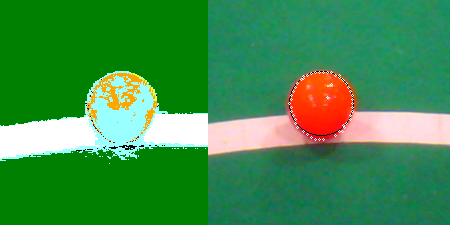
\includegraphics[width=0.5\textwidth]{figures/ballDetectionScreenshot.png}
\caption{A screenshot of the ball detection. The left image shows the colour calibrated image where a substantial proportion of the ball is unclassified (light blue), while the right shows the edge points identified and the circle fitted to the edge points.} \label{fig:ballDetection}
\end{figure}

%Figure~\ref{fig:ballDetection} shows an example of the edge-detection being used
%to accurately identify a ball. The image on the left shows the colour calibrated
%image. It can be seen that a substantial part of the ball is unclassified (note
%that unclassified colours appear as light blue in the screenshot). The image on
%the right shows that the edge-detection has enabled the edge of the ball to be
%precisely located. This is particuarly important for ball detection as kicks
%need to be lined up very precisely for them to work well.

\subsection{Goal-Post Detection}

As the majority of the goal-posts appear above the field-edge, goals are not identified during region building. Instead, x and y-axis histograms are generated while the saliency scan is built, and are used to identify the likely approximate positions of the goals, and edge-detection is then used to find the exact position of the goal-posts, or to remove false positives from the histogram stage.

This is achieved by firstly finding the maximum value in the y-axis histogram
for one of the goal colours.  Only one y coordinate is used because if there are
two goal-posts in the image, they will occupy approximately the same y
coordinate range, and the maximum in the histogram will most likely occur at a y
coordinate occupied by both posts. The x-axis histogram is then scanned to find
local maximums above a certain threshold for the goal colour. To avoid several
local maximums being detected in the same goal-post, the histogram value of the
goal-post colour has to decrease to be at least three times less than the
maximum value before another local maximum can be recorded. The same procedure
is used for both goal colours.

\begin{figure} [ht]
\centering
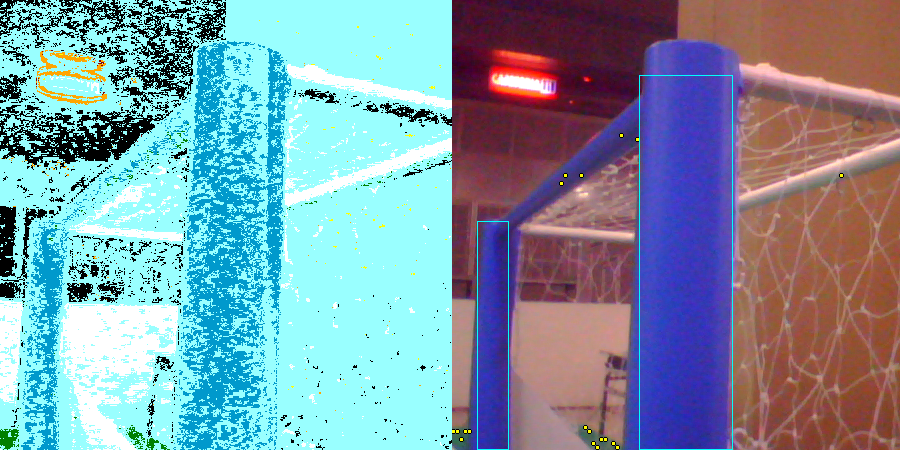
\includegraphics[width=0.6\textwidth]{figures/goalDetection.png}
\caption{Poor colour classified image of goal-posts (left). Correctly identified
goal-post using edge information (right).} \label{figGoal}
\end{figure}

Several horizontal and vertical scan-lines are used around each pair of x and y coordinates identified using the histograms. Each scan starts around the pair of x and y coordinates, and continues outwards until an edge is detected. For goal-detection, an edge is found when the two pixels differ in the sum of the differences in the \emph{y, u} and \emph{v} values by more than a certain threshold. All channels are used as the colour of the background around the goal-posts cannot be controlled, so any significant change in any channel needs to be registered as an edge. These scan-lines result in a rectangle representing the goal-post, which can then be used by the localisation algorithms. Figure~\ref{figGoal} (left) shows an example of this method.

%Figure~\ref{figGoal} (left) shows a very deteriorated colour classified image of
%the blue goal. Despite the poor quality, the foveated higher resolution
%edge-detection approach is able to clearly identify both goal-posts, as shown
%in Figure~\ref{figGoal} (right).

\section{Performance in RoboCup}

The set of algorithms presented in this paper form the cornerstone of UNSW's
visual object identification for the 2010 RoboCup competition. In this
competition, rUNSWift placed second in soccer, and first in the technical
challenges against 23 other international teams. In particular, the foveated
vision algorithm was able to successfully handle the difficult conditions of a
final game  without noticeable degradation in performance where people crowded
around the field creating significant challenges for vision by affecting the
lighting. In testing before the competition, we found that vision was able to
run at approximately 30 frames per second during game conditions.

As the region builder uses the field-edge detection to only scan the image below
the field-edge, and field-edges are used for localisation, field-edge detection
is a vital part of our vision system. We found that when the field-edge(s) could
be seen clearly, or with a few small obstructions, the field-edge detection
worked consistently and accurately. However, when there was a lot of
obstruction, such as several robots, or a referee, the field-lines were often
mis-placed. At times this caused a noticeable deterioration in the localisation
while lining up to make a kick for goals.

The advantage of using first the foveated image and virtual saccade approach
and then accurate edge-detection proved to be very beneficial to the performance
of both the goal detection and the ball detection. In following this method,
only a very small number of pixels in the saliency scan needed to be the correct
colour for the edge-detection to give an accurate match. This allowed us to
consistently and accurately detect the balls and goals, even from the opposite
side of the field, despite the large amount of colour variation due to the
curved surfaces of the goals and the ball, and various shadows on the goals.  


\section{Related Work}

A number of alternate methods have been devised to solve the complex task of object identification in the resource limited environment of RoboCup.

In order to limit the amount of interference from the background, it is often a
useful first step to identify the edge of the field in the image. Any item above
this edge can therefore be eliminated. The method used by B-Human
\cite{thomas09code} to find the edge of the field is to scan down each column in
the image to find a green segment of a minimum length, and fit a convex hull to
the start of the green segments. We imagine this approach would make the
position of the field-edge more accurate when there are a lot of non-green
objects around the edge, as RANSAC's performance deteriorates significantly with noise around the field edge. However, fitting lines to the field edge has the advantage of being easily used to localise the robot on the field.

Due to the limited processing power available on the Nao, it is not possible to
scan every pixel in the image fast enough to run in real time. An interesting
approach is taken by North\cite{north2005object}, where the density of
horizontal and vertical scan-lines is changed depending on how close the
lines are to the horizon. This uses the theory that objects close to the camera
will be large enough to be seen using extremely low resolution scan-lines, but
objects further away, near the horizon, will appear much smaller, and therefore
need a much higher density of scan-lines in order to be detected. The drawback
to this approach is that shape identification and repeated accesses are harder
and slower. This approach is also inappropriate for robots with a higher
camera, such as our 58cm Nao. In an alternate approach by Von Hundelshausen and
Rojas\cite{von2004tracking}, regions are grown from the green field, with the
white field-lines, robots and balls separating the green regions. The authors
propose that, as the robot moves, the regions can be incrementally grown and
shrunk, resulting in far fewer pixels needing to be processed and updated each
frame. This idea of using previous frames to help lower the computation time of
the current frame, while not explored in our 2010 vision system, is a worthwhile
avenue for future research, and in line with the concept of foveated imaging.

One of the most difficult parts of the object identification for robocup is the
distinction between field-lines and robots, as many parts of the robots are
white or close to white. This means that some kind of processing, other than
colour, has to be used to separate field-lines and robots. The method used by
B-Human\cite{thomas09code} to achieve this is to first create a series of small
white coloured regions that could represent either parts of a line or parts of a
robot. These regions are then analysed in terms of their shape, and ones that
more likely represent robots are marked. Finally, areas of the images where
there is a cluster of these marked regions are considered to most likely contain
robots, and every region in this area is thus removed. However this method does
not actually identify the robots.

%R\"{o}fer and J\"{u}ngel\cite{rofer2004fast} propose a different approach of
%edges and colour to achieve fast object recognition. In this method, a grid of
%horizontal and vertical scan-lines is used to search for pixels where there is a
%significant drop in the $y$ channel compared to the previous pixels searched. As
%the field is generally darker than the field-lines and the robots, this can
%indicate an edge between an object and the field. The pixels around this can
%then be colour classified to see if they are white or orange.

\section{Conclusion}

A vision processing system must be highly efficient, robust, and accurate to
enable it to perform reliably in the dynamic world of a soccer game. We have
presented a foveated imaging approach  using colour CCD cameras that can perform
the vision task in real-time. We have also presented several processor
optimisations to help improve code for low-powered embedded systems. By
utilising the hybrid modalities of colour classification and edge-detection, we
are able to reliably identify robots, goals, field-lines and balls in the
RoboCup environment. Our approach of using virtual saccades to points of
fixation of high-resolution foveal areas in the image allowed us to reduce the
processing of redundant data, and achieve processing speeds of approximately 30
frames per second in changing lighting conditions.

\bibliographystyle{plain}
\bibliography{hengst-1}

\end{document}
